\documentclass[preprint]{sigplanconf}

\usepackage[pdftex]{graphicx}
\usepackage[all]{xy}
\usepackage{tikz}
\usetikzlibrary{arrows, shapes, backgrounds, chains, decorations, calc, fit,
    shadows}
\usepackage[english]{babel}
\usepackage[Q=yes]{examplep}
\usepackage{pgf}
\usepackage{tikzuml-v1.0b/tikz-uml}
\usepackage{listings}

\lstset{
  basicstyle=\footnotesize\ttfamily
}

\begin{document}
\title{Bidirectional Git Objects Transferring by Subdirectories Specified}
\authorinfo{Congbin Guo\and Eric Wang}{VMware Inc.}{\{cguo,wange\}@vmware.com}
\maketitle
\abstract{
  % the problem
  The lack of subdirectories transferring of a Git repository (e.g. cloning,
  fetching, or pushing) consumes lots of time and network bandwidth.
  % why interesting
  This downgrades the user expierence and development efficiency against many
  large enterprise level Git repositories that have long history and huge
  amount of working files.
  % solution
  To support bidirectional transferring by subdirectories specified by a client
  from a remote repository, we extend the current Git transfer protocol to
  allow the subdirecories negotiation between server and client.
  Based on the extended protocol, we implement new server side and client side
  program to optimize Git objects transferring by removing unnecessary objects
  and replace them with special placeholders.
  The new client side program can also keep the data consistency of newly
  creatd commits.
  % value
  The proposed solution addresses the pain-point of work with large Git
  repository, helps the transistion from legacy VCS to Git, boost the adoption
  of Git in large enterprises.
}

\keywords
Git, transfer protocol, VCS, pack file, Git object model, spare
clone

\section{Introduction}
%(
% describe the problem
Git is popular but still has problems when work with large remote repositories,
which may consume lots of time and network bandwidth in data transferring from,
and to, the repository.
The reason is Git stores the history of whole workspace snapshots, which may 
have huge amount of directories and files.
The feature to only transfer subdirectories, like other popular VCS systems do
(e.g. Perforce), has been desired for long time.
But it is not in the plan of Git developers, because it may break Git
repository consistency and many Git features.
The suggestion from Git developers to deal with large repository is to break
into small ones, or omit some history by using Git shallow clone.
Neither one is very attractive to enterprise level users.

% my contribution
In this paper, we propose a solution to transfer subdirectories specified by
user from and to remote repositories efficiently.

\begin{itemize}
  \item We analyze the Git transfer protocol first, and extend it to allow
      subdirectories discovery and negotiation between server and client.
  \item Based on the extended protocol, we describe how to optimize the
      transferred data size to client by excluding some Git objects.
  \item More importantly, we discuss how to keep the newly created commits from
      the ``partial'' workspace as consistent as created from a full workspace.
\end{itemize}

%)
\section{Background}
\subsection{Git object model}
Git stores files, directories, and change histories as unique objects, i.e.
\emph{blob} \emph{tree} and \emph{commit}, with names derived from their SHA1
check sum value\cite{gitobj}.
It can be better explained by an example.
Figure \ref{fig:workspace} shows the two snapshots of a sample workspace.
\verb|file1| and \verb|file2| were modified, and a new file \verb|file4| was
added.
\begin{figure}
  \centering
  \input figures/workspace.tikz
  \caption{Snapshots of the sample workspace}
  \label{fig:workspace}
\end{figure}

Figure \ref{fig:git-repo} shows the repository.
Accordingly, there are two commit objects, $C$ and $C'$, with tip $H$ pointing
to the current version, i.e. \verb|HEAD|.
Because \verb|file3| is unchanged, the two commits share blob $B_3$.

\begin{figure}[htpb]
  \centering
  \begin{tikzpicture}[node distance=1.5cm, every node/.style={align=center}]
\input figures/git-model-base.tikz
\end{tikzpicture}

  \caption{Git repository for a sample workspace}
  \label{fig:git-repo}
\end{figure}

\subsection{Git Transfer Protocol}
%(
Current Git transfer protocol is simple and clear\cite{tran-protocol}.
The steps of transferring data from server, i.e. cloning or fetching, is shown in Figure \ref{fig:git-proto-clone-seq}:

\begin{enumerate}
  \item Client initiates the request by calling \verb|git-upload-pack| on server.
  \item Server advertises all current reference SHA1s ($H_S$) to the client.
  \item Client sends a list of SHA1 of \verb|want| ($H_w$) and \verb|have| ($H_h$), which indicates the start and end SHA1 of commit objects to be transferred.
    In case of cloning, the list of \verb|have| is skipped since the client has nothing yet.
  \item Server calculates all commit objects (and all other Git objects associated) in range of $[H_w, H_h)$, then writes to a stream connected to the client.
\end{enumerate}

\begin{figure}
  \centering
  %!tikz editor 1.0
%!tikz source begin
\begin{tikzpicture}
\begin{umlseqdiag}
\umlobject[class=Client]{c}
\umlobject[class=Server]{s}
\begin{umlcall}[op={git-upload-pack}]{c}{s}
  \begin{umlcall}[op={$H_s$}, type=return]{s}{c}
  \end{umlcall}
  \begin{umlcall}[op={$<H_w, H_h>$}, return={pack stream}]{c}{s}
    \begin{umlcall}[op={pack-objs}]{s}{s}
    \end{umlcall}
  \end{umlcall}
\end{umlcall}
\end{umlseqdiag}
\end{tikzpicture}
%!tikz source end


  \caption{Transferring Git objects from server}
  \label{fig:git-proto-clone-seq}
\end{figure}
The Git transfer protocol also covers the opposite direction, i.e. transfer
data from client to server, also known as \emph{push}.
Because it is fully reused in our solution, we don't describe it in detail
here.

\section{The problem}
To support subdirectories transferring between server and client needs to resolve below problems:
\begin{itemize}
  \item How does the client discovery the subdirectories, and negotiate with
      the server that which of them to be transferred?
  \item How does the server optimize the Git objects pack according to chosen
      subdirectories?
  \item How does the client operate with the partial Git objects store, and
      furthermore ensure the newly created commits are as good as the ones
      from fully Git objects store?
\end{itemize}
%)

\section{Solution}
Our solution includes both server side and client side changes.
\subsection{Server side}
We add two more steps in server side, one is negotiating subdirectories, another is excluding uninterested objects from packing.
\subsubsection{Subdirectories Negotiation}
Client can send all subdirectories interested and excluded when it has enough information.
Otherwise, the negotiation is necessary.
The subdirectories negotiation is an interactive process because the client may know nothing about the directories, especially in cloning.

We add an extra step in the standard transfer protocol to allow subdirectories negotiation between client and server.
The step is initiated by client, so it's transparent for common Git client, which can ensure the server compatibility for all kinds of client.
\begin{figure}
  \centering
  %!tikz editor 1.0
%!tikz source begin
\begin{tikzpicture}
\begin{umlseqdiag}                                                             
\umlobject[class=Client]{c}                                                    
\umlobject[class=Server]{s}                                                    
\begin{umlcall}[op={git-upload-pack}, return={pack stream}]{c}{s}
    \begin{umlcall}[op={$H_S$}, type=return]{s}{c}
    \end{umlcall} 
    \begin{umlfragment}[type=loop]
        \begin{umlcall}[op={dir}]{c}{s}
        \end{umlcall}
        \begin{umlcall}[op={$D_S$}, type=return]{s}{c}
        \end{umlcall}
    \end{umlfragment}
    \begin{umlcall}[op={$<H_h, H_w, D_i, D_e>$}]{c}{s}
    \end{umlcall}
    \begin{umlcall}[op={pack_objs($[H_s, H_c), D_i, D_e$)}]{s}{s}
    \end{umlcall}                 
\end{umlcall}  
\end{umlseqdiag}
\end{tikzpicture}
%!tikz source end


  \caption{Extended Git transfer protocol}
  \label{fig:git-proto-ext-seq}
\end{figure}

Operations and server response


The extension includes three primitive commands.
\begin{itemize}
  \item \verb|dir| get directory of a SHA1:path.
    this is equivalent to command \verb|git ls-tree SHA1 -- path|.
    Server returns a list of files or directories under the path specified.
  \item \verb|include| used to specify which subdirectories will be included in result.
  \item \verb|exclude| used to specify which subdirectories should be excluded from result.
\end{itemize}

\begin{figure}
  \centering
  \begin{verbatim}
  upload-request = dir-commands
                   want-list
                   have-list
                   compute-end

  dir-commands = *dir-command

  dir-command = PKT-LINE(dir SP obj-id SP path LF)
  \end{verbatim}
  \caption{Extended Git transfer protocol ABNF}
  \label{fig:git-proto-ext-ABNF}
\end{figure}

The server response of \verb|dir| command is same with command of 
\verb|git ls-tree|. 
\begin{figure}
  \centering
  \begin{verbatim}
  advertised-dirs = dir-list
                    flush-pkt

  dir-list = *(dir-line)

  dir-line = PKT-LINE(mode SP type SP obj-id \
                      TAB name LF)

  type = tree | blob
  \end{verbatim}
  \caption{Server response in ABNF}
  \label{fig:server-response-ABNF}
\end{figure}
The BNF of those three commands.
...

\subsubsection{Packing Objects Optimization}
In standard Git protocol, the object packing can be regards as a piped command, i.e.
\begin{verbatim}
git-rev-list|git-pack-objects
\end{verbatim}
That is, get a list of all commits (and its associated objects) first, then pack them.

We try to transfer fewer objects to save time and system resources.
But which objects can be removed from the packing list?
We must keep commit and tag objects for repository consistency.
So only tree and blob objects can be excluded, if they are not in the subdirectories client want.

In the sample repository shown in Figure \ref{fig:git-repo}, suppose the client only want \verb|file1| (represented as $B_1$ and $B'_1$).
The candidate objects for excluding are tree objects ($T_1$ and $T'_1$), and blob objects ($B_2$, $B'_2$, $B_3$ and $B_4$), as highlighted in Figure \ref{fig:find-obj-to-remove}.
\begin{figure}[htpb]
  \centering
  \begin{tikzpicture}[node distance=1.5cm, every node/.style={align=center}]
\input figures/git-model-base.input
\begin{pgfonlayer}{background}
  \node[ellipse, fill=black!20, fit=(tr1_1) (b1_2) (b1_3), xscale=0.75,
  yshift=-0.5cm]{};
  \node[ellipse, fill=black!20, fit=(tr2_1) (b2_2) (b2_4)]{};
\end{pgfonlayer}
\end{tikzpicture}

  \caption{Objects can be excluded in the sample repository}
  \label{fig:find-obj-to-remove}
\end{figure}

After that, we have a reduced object list, and pass that to \verb|git-pack-objects| command to pack.
The whole process can be regarded as a command as:
\begin{verbatim}
git-rev-list|filter($D_i$, $D_e$)|git-pack-objects
\end{verbatim}

\subsection{Client side}
\subsubsection{Packing Objects Receiving}
The pack stream transferred to the client can not be handled by Git directly due to the excluded objects.
We create placeholder files in client for the excluded ones, which we call \emph{Git mock objects}.
The mock objects have same name, i.e. the SHA1 string of the object, as the original objects.
But the content of mock objects is empty.

The reason why we can use empty file as the placeholder is because that Git performs consistency checks based on SHA1 values get from the object file name, rather than re-calculate it again from the content. In other words, Git only cares about the object file name instead of the content.

Figure \ref{fig:cmd-create-mock} shows one way to create empty blob and tree object by command line.
The object file prefixed with \verb|e69de29| and \verb|4b825dc| are the mock blob and tree object we want.
They can play the placeholder to any same type Git object by just renaming it to target SHA1.
The benefits of using those mock objects are:
\begin{enumerate}
  \item They are still Git objects with correct format, though named with SHA1 string of another object.
  \item Their size is small and easy to be created.
  \item An empty tree object can dereference all associated objects, eliminating the need for placeholders for sub-trees and blobs.
\end{enumerate}


\begin{figure}[htpb]
  \centering
  \begin{verbatim}
    # create an empty blob object
    $ :> empty_file
    $ git hash-object -w empty_file
    e69de29bb2d1d6434b8b29ae775ad8c2e48c5391

    # create an empty tree object
    $ git mktree <<EOF
    EOF
    4b825dc642cb6eb9a060e54bf8d69288fbee4904
  \end{verbatim}
  \caption{Command line to create Git mock objects}
  \label{fig:cmd-create-mock}
\end{figure}

Figure \ref{fig:mock-objects} shows the resulting diagram with the mock objects.

\begin{itemize}
  \item The mock object $B_m$ replaces the blob object $B_4$.
  \item The mock tree object $T_m$ and $T'_m$ replace two tree objects, $T_2$ and $T'_2$.
\end{itemize}

\begin{figure}[htpb]
  \centering
  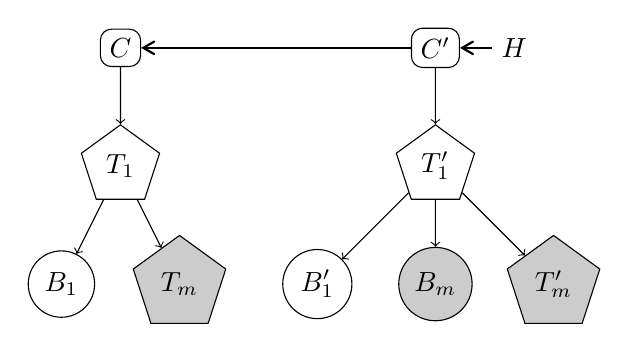
\begin{tikzpicture}
\tikzstyle{commit}=[rectangle, draw, rounded corners]
\tikzstyle{tree}=[regular polygon, regular polygon sides=5, draw, thin]
\tikzstyle{blob}=[circle, draw, thin]

% mock tree/blob object
\tikzstyle{mock_tree}=[regular polygon, regular polygon sides=5, draw, thin,
  fill=black!20]
\tikzstyle{mock_blob}=[circle, draw, thin, fill=black!20]

\tikzstyle{parent}=[-angle 60, draw, thick]
\tikzstyle{edge from parent}=[->, draw]
\tikzstyle{2obj}=[->, draw]
% tree 1
\node[commit](ci1){$C$}
child{node[tree](tr1){$T_1$}
  child{node[blob](b1_1){$B_1$}}
  child{node[mock_tree](tr1_1){$T_m$}}
};

% tree 2
\node[commit, right of=ci1, node distance=4cm](ci2){$C'$}
child{node[tree](tr2){$T'_1$}
  child{node[blob](b2_1){$B'_1$}}
  child{node[mock_blob](b2_4){$B_m$}}
  child{node[mock_tree](tr1_1){$T'_m$}}
};

\draw[parent](ci2) to (ci1);


% HEAD
\node[rectangle, right of=ci2](head){$H$};
\draw[parent](head) to (ci2);


\end{tikzpicture}

  \caption{Replacing Git objects with mock objects}
  \label{fig:mock-objects}
\end{figure}

With those mock objects, Git does not complain anything about the data from the server.

\subsubsection{Workspace Checking-out}
Like normal Git objects, the mock objects can also be checked out to workspace.
The checked-out mock blob objects is a empty file.
And the checked-out mock tree object is nothing.

The checking out of those mock objects can make Git think the current workspace is dirty.
That is because Git recalculates the SHA1 value of working files and compare what recorded in Git index.
Obviously, they are different.

We use \emph{Git sparse checkout} \cite{sparseco} to avoid that, which only
checkout specified subdirectories from repository into workspace.
Here we can reuse the result of subdirectories negotiation done before.
That is what user really want to get initially.



\subsubsection{New Commits Creating}
Git staging area, or \emph{index}, which generally kept in \verb|.git/index|,
is the key data structure for Git to prepare a new commit.
It contains a sorted list of all path names of current tree, each with
permissions and the SHA1 of a blob object \cite{idx-format}.
Git uses the data stored in index to create a tree object, then creates a
commit with that tree.
Even for Git sparse checking out, in which only a part of files be checked
out, the index still contains a full list of all files for committing.

In our case, nothing can be loaded to Git index by reading mock tree objects
since they are empty.
This results in partial Git index which cannot work properly when creating new
commits, which all directories represented by mock tree objects regarded as
removed.

Because it makes no sense for users to modify files out of the scope of
subdirectories negotiated in our solution, we extract missing blob and tree
objects information from the most recent commit, and combine it with data
stored in the Git index to form a complete tree object, then rewrite the commit
to point to the complete tree object.
We do the rewriting just after every new commit created.
Below is the more detail steps:

\begin{enumerate}
  \item Get the tree object content of current version $T_h$, i.e. \\
        \verb|git cat-file -p HEAD^{tree}|.
  \item Get staging files path and SHA1 information $T_t$ from Git index.
  \item Combine the content of $T_h$ and $T_t$ together, then construct a new
        tree object $T$ by command \verb|git mktree|.
  \item Run command \verb|git commit-tree |$T$ to create a new commit object
        $C$.
  \item Update current branch tip to pointed to $C$ by command \\
        \verb|git update-ref|.
\end{enumerate}




\section{The details}
\subsection{The Implementation}
We developed a prototype to prove the solution works.

\subsection{Experiment}
We had a basic experiment to measure teh performanc of the prototype.
Though the prototype was not fully optimized, we still saw sustantial
performance improvements in both the Git objects store size and the time to
transfer it.

The repo we used is a Git mirror of a perforce depot, i.e.
\verb|mirrors/vmware/perforce-1666_bora_prod-2015.git| from
\verb|git.eng.vmware.com|.

In the experiment, we performed four operations:
\begin{itemize}
  \item \emph{full clone}: clone the entire repository by standard clone
    command.
  \item \emph{sparse clone 1}: only clone the \verb|README| file.
  \item \emph{sparse clone 2}: only clone the \verb|README| file and the
  \verb|doc/| directory.
  \item \emph{sparse clone 3}: clone all files and directories which is the
    worst case.
\end{itemize}
Table \ref{tbl:repo-info} shows the static data of repositories cloned.



\section{Related work}
E. Newren did some inspiring work in \cite{newren10-0}, \cite{newren10-1},
which describes the idea of just clone referenced objects to client side.
Additionally, this work also uses \emph{git replace} mechanism to deal with
commit history.
However, due to modification to cloned commits and index file, some common Git
important operations cannot work perfectly, such as fetch, push, rebase, etc.

N. Duy has also begun to work on sparse clone or subtree clone since 2008; and
who submitted a series of patch in Git community.
\cite{duy08}, \cite{duy10-1}, \cite{duy10-2}, and \cite{duy10-3} describes a
sparse clone method by adding an extra option to \verb|git clone| command, and
rewriting/replacing the commits in clone time.
The work also has pointed out the performance limitation of Git replacement
mechanism.
The weak part of the work is multiple directories cannot be fully supported.

\section{Limitations}
Because of changing in Git object store, the implementation cannot support
any Git operations care about repository, e.g. the command of \verb|fsck|,
\verb|repack|, and \verb|gc|.
Additionally, since the mock tree object is empty, running the command of
\verb|ls-tree| or \verb|cat-file| on that tree object produces empty output.

Another limitation is, since the Git index is partial comparing with normal Git
clone, commands related to Git index may give different results, e.g.
\verb|git ls-files|.





\begin{thebibliography}{10}
    \softraggedright

    \bibitem{sparseco} \emph{Git-read-tree(1) Manual Page} (February
      2013). \newblock URL
      [https://www.kernel.org/pub/software/scm/git/docs/git-read-tree.html]
    \bibitem{roadmap} J. Hamano (July 2008). \newblock \emph{sparse fetch}.
    \newblock Git mailing list. \newblock URL
      [http://thread.gmane.org/gmane.comp.version-control.git/89681/focus=90016]
    \bibitem{gitobj} S. Chacon (July 2009).\newblock\emph{Pro Git}, section 9.2.
      \newblock URL
      [http://git-scm.com/book/en/Git-Internals-Git-Objects]
      \bibitem{idx-format} \emph{GIT index format}.\newblock URL
      https://www.kernel.org/pub/software/scm/git/docs/technical/index-format.txt
    \bibitem{packformat} \emph{GIT pack format}.\newblock URL
      [https://www.kernel.org/pub/software/scm/git/docs/technical/pack-format.txt]
    \bibitem{replace} \emph{git-replace(1) Manual Page} (February 2013).\newblock
      URL [https://www.kernel.org/pub/software/scm/git/docs/git-replace.html]
    \bibitem{tran-protocol} \emph{Pack files transfer protocol}.\newblock URL
      [https://www.kernel.org/pub/software/scm/git/docs/v1.7.0.5/technical/\\
      pack-protocol.txt]
    \bibitem{duy08}N. Duy (July 2008).\newblock \emph{git-clone: support --path
      to do sparse clone}. \newblock Git mailing list. \newblock URL
      [http://article.gmane.org/gmane.comp.version-control.git/89681]
    \bibitem{newren10-0}E. Newren (July 2010). \newblock \emph{Sparse clones}.
      \newblock Git mailing list. \newblock URL
      http://article.gmane.org/gmane.comp.version-control.git/152020
    \bibitem{newren10-1}E. Newren (September 2010). \newblock \emph{Sparse
      clones}.  \newblock Git mailing list. \newblock URL
      http://article.gmane.org/gmane.comp.version-control.git/155389
    \bibitem{duy10-1}N. Duy (July 2010). \newblock \emph{Subtree clone?}. \newblock
      Git mailing list. \newblock URL
      [http://article.gmane.org/gmane.comp.version-control.git/151937]
    \bibitem{duy10-2}N. Duy (July 2010). \newblock \emph{Subtree clone proof of
    concept}. \newblock Git mailing list. \newblock URL
    [http://article.gmane.org/gmane.comp.version-control.git/152347].
    \bibitem{duy10-3}N. Duy (August 2010). \newblock \emph{subtree clone v2}.
    \newblock Git mailing list. \newblock
    URL [http://article.gmane.org/gmane.comp.version-control.git/154343].
\end{thebibliography}

\end{document}

